\documentclass[aspectratio=169,11pt,t]{beamer}

% ============================================================
% Theme and typography
% ============================================================

\usetheme{Madrid}
\usecolortheme{default}
\usefonttheme{professionalfonts}

\setbeamertemplate{navigation symbols}{}
\setbeamertemplate{headline}{}

\setbeamertemplate{footline}{%
  \leavevmode\hbox{%
  \begin{beamercolorbox}[wd=.82\paperwidth,ht=2.5ex,dp=1.0ex,leftskip=.8em]{author in head/foot}
    CSCI 6461 --- Computer Systems Architecture
  \end{beamercolorbox}%
  \begin{beamercolorbox}[wd=.18\paperwidth,ht=2.5ex,dp=1.0ex,rightskip=.8em]{date in head/foot}
    \hfill\insertframenumber/\inserttotalframenumber
  \end{beamercolorbox}}
}

\setbeamersize{
  text margin left=0.65cm,
  text margin right=0.65cm
}

\setbeamerfont{frametitle}{size=\Large, series=\bfseries}
\setbeamerfont{block title}{size=\normalsize, series=\bfseries}
\setbeamertemplate{blocks}[rounded][shadow=false]

% Block vertical padding adjustments
\addtobeamertemplate{block begin}{\vspace{0.1em}}{\vspace{0.1em}}
\addtobeamertemplate{block end}{}{\vspace{0.2em}}

% Base list item separation
\setbeamertemplate{itemize/enumerate body begin}{\setlength{\itemsep}{4pt}}
\setbeamertemplate{itemize/enumerate subbody begin}{\setlength{\itemsep}{2pt}}

% ============================================================
% Packages
% ============================================================

\usepackage[T1]{fontenc}
\usepackage{lmodern}
\IfFileExists{sourcecodepro.sty}
  {\usepackage[scale=0.92]{sourcecodepro}}
  {\usepackage{courier}}
\usepackage{amsmath}
\usepackage{booktabs}
\usepackage{array}
\usepackage{colortbl}
\usepackage{tikz}

\usetikzlibrary{
  arrows.meta,
  positioning,
  shapes.geometric,
  calc,
  decorations.pathreplacing
}

% ============================================================
% Colors
% ============================================================

\definecolor{navy}{RGB}{24,43,68}
\definecolor{deepblue}{RGB}{45,88,130}
\definecolor{lightblue}{RGB}{235,242,250}
\definecolor{softgray}{RGB}{245,247,250}
\definecolor{darkgray}{RGB}{25,28,32}
\definecolor{gold}{RGB}{200,145,35}

\setbeamercolor{palette primary}{bg=navy,fg=white}
\setbeamercolor{palette secondary}{bg=deepblue,fg=white}
\setbeamercolor{frametitle}{bg=navy,fg=white}
\setbeamercolor{title}{fg=white}
\setbeamercolor{subtitle}{fg=white}
\setbeamercolor{author}{fg=white}
\setbeamercolor{date}{fg=white}
\setbeamercolor{titlelike}{fg=white}
\setbeamercolor{block title}{bg=deepblue,fg=white}
\setbeamercolor{block body}{bg=lightblue,fg=darkgray}
\setbeamercolor{normal text}{fg=darkgray,bg=white}

% ============================================================
% Formatting shortcuts
% ============================================================

\setlength{\parskip}{0pt}

\newcommand{\key}[1]{\textbf{#1}}
\newcommand{\bits}[1]{\texttt{#1}}
\newcommand{\hex}[1]{\texttt{0x#1}}
\newcommand{\code}[1]{\texttt{#1}}

% Section divider macro
\newcommand{\sectiondivider}[2]{%
\begin{frame}[plain]

\begin{tikzpicture}[remember picture,overlay]
\fill[navy] (current page.south west) rectangle (current page.north east);
\fill[gold] (current page.south west)
  rectangle ([yshift=.15cm]current page.south east);
\end{tikzpicture}

\vspace*{\fill}

\begin{minipage}{0.94\textwidth}
\raggedright
\hyphenpenalty=10000
\exhyphenpenalty=10000

{\color{gold}\large\bfseries #1\par}

\vspace{0.3cm}

{\color{white}\fontsize{22}{26}\selectfont\bfseries
#2\par}

\end{minipage}

\vspace*{\fill}

\end{frame}
}

% ============================================================
% Metadata
% ============================================================

\title[Topic 5]{
  Memory Architecture \& Addressing Principles
}

\subtitle{
  The load/store model, address computation, data sizing,\\
  and memory hierarchy interactions in AArch64
}

\author{
  Computer Systems Architecture
}

\date{}

% ============================================================
% Document
% ============================================================

\begin{document}





% ============================================================
% Slide 1
% ============================================================

\begin{frame}[plain]
\begin{tikzpicture}[remember picture,overlay]
\fill[navy] (current page.south west) rectangle (current page.north east);
\fill[gold] (current page.south west) rectangle ([yshift=.15cm]current page.south east);
\end{tikzpicture}

\vspace{0.8cm}
\begin{minipage}{0.88\textwidth}
{\color{gold}\normalsize\bfseries CSCI 6461 \;|\; TOPIC 5\par}
\vspace{0.25cm}
{\color{white}\fontsize{24}{28}\selectfont\bfseries
 Memory Architecture\\[0.08cm]
 \& Addressing Principles
\par}
\vspace{0.35cm}
{\color{white!80}\large
 The load/store model, address computation, data sizing,\\
 and memory hierarchy interactions in AArch64
\par}
\end{minipage}

\vfill
{\color{white}\normalsize Dr. J. Burns\par}
{\color{white!70}\small Computer Systems Architecture --- AArch64 Reference Platform\par}
\vspace{0.35cm}
\end{frame}






% ============================================================
% Slide 2
% ============================================================


\begin{frame}{Topic 5 Outline}

\setbeamertemplate{enumerate item}{\arabic{enumi}.}
\begin{enumerate}\setlength{\itemsep}{10pt}
  \item \key{Memory Access and Computation}
  \begin{itemize}
    \item Why AArch64 separates memory transfers from arithmetic operations.
    \item How values move between memory and the register file.
  \end{itemize}

  \item \key{Data Types, Widths, and Conversions}
  \begin{itemize}
    \item Handling bytes, halfwords, words, and doublewords cleanly.
    \item Choosing zero-extension or sign-extension when loading sub-word data.
  \end{itemize}

  \item \key{Address Calculation}
  \begin{itemize}
    \item Immediate offsets, pre/post-indexing, and scaled array indexing.
    \item How each addressing form changes, or does not change, the base register.
  \end{itemize}

  \item \key{Applied Access Patterns}
  \begin{itemize}
    \item Practical array traversal and indexed-array access patterns.
    \item Choosing the addressing form that matches the data-access pattern.
  \end{itemize}
\end{enumerate}

\end{frame}



% ============================================================
% Section 1 Divider
% ============================================================

\sectiondivider{PART 1}{The Load/Store Architectural Boundary}





% ============================================================
% Slide 3
% ============================================================


\begin{frame}{The Fundamental Memory Challenge}
\large
\begin{itemize}\setlength{\itemsep}{7pt}
  \item Registers are fast but limited in number; memory holds much more data but is accessed through explicit transfer instructions.
  \item \key{Architectural Question:} How should the instruction set organize data movement between memory and the register file?
  \item AArch64 uses a strict \key{load/store discipline}: ALU instructions operate on registers, while load/store instructions access memory.
\end{itemize}

\vspace{0.35cm}
\begin{block}{The Architectural Rule}
ALU instructions process \emph{only} register operands. Memory access is performed by load/store-family instructions.
\end{block}
\end{frame}






% ============================================================
% Slide 4
% ============================================================


\begin{frame}{Separating Computation from Data Movement}

\begin{columns}[T,onlytextwidth]
\begin{column}{0.48\textwidth}
\begin{block}{Architectural Separation}
\begin{itemize}\setlength{\itemsep}{4pt}
  \item Arithmetic instructions do not directly access data memory.
  \item Load instructions copy values from memory into registers.
  \item Store instructions copy register values back to memory.
\end{itemize}
\end{block}
\end{column}

\begin{column}{0.48\textwidth}
\begin{block}{Typical Data Flow}
\begin{enumerate}\setlength{\itemsep}{3pt}
  \item \key{Load:} bring data into registers.
  \item \key{Compute:} operate on register values.
  \item \key{Store:} write the result back if needed.
\end{enumerate}
\end{block}
\end{column}
\end{columns}

\vspace{0.4cm}
\centering
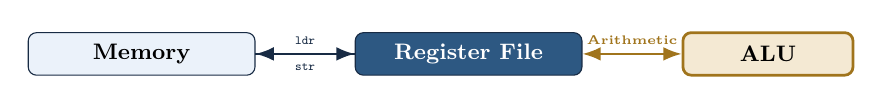
\begin{tikzpicture}[scale=0.9, every node/.style={transform shape}]
  \node[draw=navy, fill=lightblue, rounded corners=3pt, font=\small\bfseries, minimum width=3.2cm, minimum height=0.6cm] (mem) {Memory};
  \node[draw=navy, fill=deepblue, text=white, rounded corners=3pt, font=\small\bfseries, right=1.4cm of mem, minimum width=3.2cm, minimum height=0.6cm] (reg) {Register File};
  \node[draw=gold!80!black, fill=gold!20, line width=1pt, rounded corners=3pt, font=\small\bfseries, right=1.4cm of reg, minimum width=2.4cm, minimum height=0.6cm] (alu) {ALU};

  \draw[-{Latex}, thick, navy] (mem) -- (reg) node[midway, above, font=\tiny\bfseries] {\code{ldr}};
  \draw[-{Latex}, thick, navy] (reg) -- (mem) node[midway, below, font=\tiny\bfseries] {\code{str}};
  \draw[{Latex}-{Latex}, thick, gold!80!black] (reg) -- (alu) node[midway, above, font=\tiny\bfseries] {Arithmetic};
\end{tikzpicture}
\end{frame}






% ============================================================
% Slide 5
% ============================================================







% ============================================================
% Slide 6
% ============================================================


\begin{frame}{Addressing Memory: Bytes, Words, and Doublewords}
\large
\begin{itemize}\setlength{\itemsep}{6pt}
  \item Memory is a linear sequence of \key{8-bit bytes}; each byte has its own address.
  \item The instruction/access size determines the transfer width:
\end{itemize}

\vspace{0.2cm}
\begin{center}
\small
\setlength{\tabcolsep}{8pt}
\begin{tabular}{lccc}
\toprule
\textbf{Data Type} & \textbf{Width} & \textbf{Load Syntax} & \textbf{Store Syntax} \\
\midrule
Byte         & 8-bit   & \code{ldrb wt, [xn]} & \code{strb wt, [xn]} \\
Halfword     & 16-bit  & \code{ldrh wt, [xn]} & \code{strh wt, [xn]} \\
Word         & 32-bit  & \code{ldr  wt, [xn]} & \code{str  wt, [xn]} \\
Doubleword   & 64-bit  & \code{ldr  xt, [xn]} & \code{str  xt, [xn]} \\
\bottomrule
\end{tabular}
\end{center}

\vspace{0.25cm}
\normalsize
The base register (\bits{xn}) holds the memory pointer enclosed in brackets: \code{[xn]}.
\end{frame}


% ============================================================
% Section 2 Divider
% ============================================================

\sectiondivider{PART 2}{Data Sizing \& Extension Rules}





% ============================================================
% Slide 7
% ============================================================


\begin{frame}{Sub-Word Loads and Extension}
\large
\begin{itemize}\setlength{\itemsep}{7pt}
  \item Registers are 64 bits wide, but memory values may be only 8, 16, or 32 bits.
  \item When a smaller value is loaded, the processor must fill the remaining upper bits.
  \item The correct choice depends on whether the memory value should be treated as \key{unsigned} or \key{signed}.
\end{itemize}

\vspace{0.25cm}
\begin{columns}[T,onlytextwidth]
\begin{column}{0.48\textwidth}
\begin{block}{Zero-Extension}
Use for unsigned data. Upper bits are filled with \bits{0}s.
\end{block}
\end{column}

\begin{column}{0.48\textwidth}
\begin{block}{Sign-Extension}
Use for signed data. The sign bit is copied into the upper bits.
\end{block}
\end{column}
\end{columns}
\end{frame}






% ============================================================
% Slide 8
% ============================================================







% ============================================================
% Slide 9
% ============================================================







% ============================================================
% Slide 10
% ============================================================


\begin{frame}{Sign vs.\ Zero Extension: Side-by-Side}
\begin{block}{Memory Byte at Address \texttt{x1} = \hex{80} (Binary: \texttt{1000 0000})}
The same 8-bit pattern means either unsigned \(128\) or signed \(-128\), depending on the load instruction.
\end{block}

\vspace{0.15cm}
\begin{center}
\footnotesize
\setlength{\tabcolsep}{6pt}
\begin{tabular}{ll>{\raggedright\arraybackslash}p{5.8cm}}
\toprule
\textbf{Instruction} & \textbf{Value in \texttt{x0}} & \textbf{Meaning} \\
\midrule
\code{ldrb  w0, [x1]} & \texttt{0x00000000\_00000080} & Zero-extends the byte; interpreted as unsigned \(+128\). \\
\code{ldrsb x0, [x1]} & \texttt{0xffffffff\_ffffff80} & Sign-extends the byte; preserves signed value \(-128\). \\
\bottomrule
\end{tabular}
\end{center}

\vspace{0.25cm}
\normalsize
Using a zero-extending load for signed negative data can turn a negative value into a large positive one.
\end{frame}






% ============================================================
% Slide 11
% ============================================================

\begin{frame}{Storing Data: Truncation Rules}
\large
\begin{itemize}\setlength{\itemsep}{6pt}
  \item Stores move data from a register into memory.
  \item The instruction width determines how many bytes from the register are written:
\end{itemize}

\vspace{0.15cm}
\begin{center}
\small
\setlength{\tabcolsep}{8pt}
\begin{tabular}{lll}
\toprule
\textbf{Instruction} & \textbf{Bits Read from Register} & \textbf{Bytes Written to Memory} \\
\midrule
\code{strb wt, [xn]} & Bits [7:0]   & Writes exactly 1 byte \\
\code{strh wt, [xn]} & Bits [15:0]  & Writes exactly 2 bytes \\
\code{str  wt, [xn]} & Bits [31:0]  & Writes exactly 4 bytes \\
\code{str  xt, [xn]} & Bits [63:0]  & Writes full 8 bytes (doubleword) \\
\bottomrule
\end{tabular}
\end{center}

\vspace{0.25cm}
\normalsize
Storing a byte or halfword modifies \emph{only} the targeted memory locations; neighboring bytes are left unchanged.
\end{frame}

% ============================================================
% Section 3 Divider
% ============================================================

\sectiondivider{PART 3}{AArch64 Addressing Modes}





% ============================================================
% Slide 12
% ============================================================

\begin{frame}{Addressing Modes}
\large
\begin{itemize}\setlength{\itemsep}{6pt}
  \item An \key{addressing mode} is how a load/store instruction forms the memory address it will access.
  \item The resulting address is the \key{effective address}: the actual byte address used by the load or store.
\end{itemize}

\vspace{0.2cm}
\begin{center}
\small
\setlength{\tabcolsep}{7pt}
\rowcolors{2}{softgray}{white}
\begin{tabular}{lll}
\toprule
\rowcolor{white}
\textbf{Access Pattern} & \textbf{Addressing Form} & \textbf{Typical Use} \\
\midrule
Fixed offset from a base pointer & \code{[xn, \#imm]} & Struct fields, known offsets \\
Step through consecutive elements & \code{[xn], \#imm} & Array traversal \\
Base plus scaled index & \code{[xn, xm, lsl \#k]} & \code{arr[i]} access \\
\bottomrule
\end{tabular}
\end{center}

\vspace{0.18cm}
\normalsize
The key question is whether the offset is fixed, index-based, or part of a pointer update.
\end{frame}





% ============================================================
% Slide 13
% ============================================================

\begin{frame}{Mode 1: Base Register with Immediate Offset}

\begin{itemize}\setlength{\itemsep}{5pt}
  \item Adds a fixed constant to a base pointer without modifying the base register.
  \item \key{Syntax:} \code{ldr xt, [xn, \#offset]} $\implies \text{EA} = x_n + \text{offset}$.
\end{itemize}

\vspace{0.2cm}
\centering
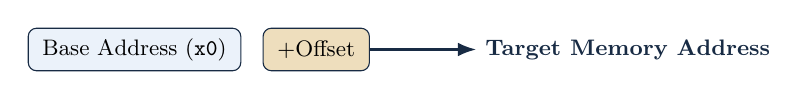
\begin{tikzpicture}[scale=0.9, every node/.style={transform shape}]
  \node[draw=navy, fill=lightblue, rounded corners=3pt, font=\small, minimum width=3.0cm, minimum height=0.6cm] (base) {Base Address (\bits{x0})};
  \node[draw=navy, fill=gold!30, rounded corners=3pt, font=\small, right=0.3cm of base, minimum width=1.5cm, minimum height=0.6cm] (off) {$+ \text{Offset}$};
  \draw[-{Latex}, thick, navy] (off.east) -- ++(1.5,0) node[right, font=\small\bfseries] {Target Memory Address};
\end{tikzpicture}

\vspace{0.3cm}
\begin{block}{Example: Reading Struct Fields}
\small
\begin{tabular}{ll}
\code{ldr x1, [x0, \#0]}  & \text{\scriptsize // Read field 1 at offset 0} \\
\code{ldr x2, [x0, \#8]}  & \text{\scriptsize // Read field 2 at offset 8} \\
\code{ldr w3, [x0, \#16]} & \text{\scriptsize // Read 32-bit field at offset 16} \\
\end{tabular}
\end{block}
\end{frame}





% ============================================================
% Slide 14
% ============================================================


\begin{frame}{Scaled Immediate Offsets}
\large
\begin{itemize}\setlength{\itemsep}{6pt}
  \item Some load/store offsets are scaled by the size of the access.
  \item For a 64-bit load, an offset of \code{\#8} means one doubleword past the base address.
  \item For a 32-bit load, an offset of \code{\#4} means one word past the base address.
\end{itemize}

\vspace{0.25cm}
\begin{block}{Conceptual Rule}
The offset tells the instruction where the desired object is relative to the base pointer. The instruction width tells the processor how many bytes to transfer.
\end{block}
\end{frame}






% ============================================================
% Slide 15
% ============================================================

\begin{frame}{Mode 2: Pre-Indexed Addressing (Update Before Access)}

\begin{itemize}\setlength{\itemsep}{5pt}
  \item Updates the base register \key{before} reading or writing memory.
  \item \key{Syntax:} \code{ldr xt, [xn, \#offset]!} \quad (Exclamation mark indicates update).
\end{itemize}

\vspace{0.2cm}
\begin{block}{Step-by-Step Action}
\begin{enumerate}\setlength{\itemsep}{3pt}
  \item $x_n \leftarrow x_n + \text{offset}$ \quad (Update pointer)
  \item Access memory at the \key{new} address in $x_n$.
\end{enumerate}
\end{block}

\vspace{0.25cm}
\begin{block}{Primary Use Case: Access After Pointer Adjustment}
\code{ldr x0, [x1, \#-8]!} \\
\text{\scriptsize Moves the base pointer back by 8 bytes, then loads from the updated address.}
\end{block}
\end{frame}





% ============================================================
% Slide 16
% ============================================================

\begin{frame}{Mode 3: Post-Indexed Addressing (Update After Access)}

\begin{itemize}\setlength{\itemsep}{5pt}
  \item Reads or writes memory at the current address, then updates the base pointer \key{afterwards}.
  \item \key{Syntax:} \code{ldr xt, [xn], \#offset} \quad (Offset written outside the brackets).
\end{itemize}

\vspace{0.2cm}
\begin{block}{Step-by-Step Action}
\begin{enumerate}\setlength{\itemsep}{3pt}
  \item Access memory at the \key{current} address in $x_n$.
  \item $x_n \leftarrow x_n + \text{offset}$ \quad (Advance pointer)
\end{enumerate}
\end{block}

\vspace{0.25cm}
\begin{block}{Primary Use Case: Array Stepping}
\code{ldr x0, [x1], \#8} \\
\text{\scriptsize Loads data from the current address in x1, then automatically advances x1 to the next 8-byte element.}
\end{block}
\end{frame}





% ============================================================
% Slide 17
% ============================================================

\begin{frame}{Comparing the Three Offset Modes}
\begin{center}
\small
\setlength{\tabcolsep}{6pt}
\begin{tabular}{llll}
\toprule
\textbf{Mode} & \textbf{Syntax Pattern} & \textbf{Address Accessed} & \textbf{Base Register After} \\
\midrule
\textbf{Standard Offset} & \code{[xn, \#8]}  & $x_n + 8$ & $x_n$ (Unchanged) \\
\textbf{Pre-Indexed}     & \code{[xn, \#8]!} & $x_n + 8$ & $x_n + 8$ (Updated) \\
\textbf{Post-Indexed}    & \code{[xn], \#8}  & $x_n$     & $x_n + 8$ (Updated) \\
\bottomrule
\end{tabular}
\end{center}

\vspace{0.3cm}
\begin{block}{Assume \texttt{x1} = \hex{1000} Initially}
\small
\begin{tabular}{llll}
\code{ldr x0, [x1, \#8]}  & $\implies$ Reads from \hex{1008}; & $x_1$ remains \hex{1000} \\
\code{ldr x0, [x1, \#8]!} & $\implies$ Reads from \hex{1008}; & $x_1$ becomes \hex{1008} \\
\code{ldr x0, [x1], \#8}  & $\implies$ Reads from \hex{1000}; & $x_1$ becomes \hex{1008} \\
\end{tabular}
\end{block}
\end{frame}





% ============================================================
% Slide 18
% ============================================================

\begin{frame}{Mode 4: Register Offset with Scaling}
\large
\begin{itemize}\setlength{\itemsep}{6pt}
  \item Uses an index register ($x_m$) multiplied by element size to access array items:
  $$\code{ldr xt, [xn, xm, lsl \#shift]}$$
  \item The instruction encodes the scaled register offset directly, though implementation latency depends on the processor.
\end{itemize}

\vspace{0.2cm}
\begin{center}
\small
\setlength{\tabcolsep}{8pt}
\begin{tabular}{lll}
\toprule
\textbf{Array Element Type} & \textbf{Assembly Instruction} & \textbf{Effective Address} \\
\midrule
Byte (\code{uint8})    & \code{ldrb w0, [x1, x2]}          & $\text{EA} = x_1 + x_2$ \\
Halfword (\code{uint16})& \code{ldrh w0, [x1, x2, lsl \#1]} & $\text{EA} = x_1 + (x_2 \times 2)$ \\
Word (\code{uint32})    & \code{ldr  w0, [x1, x2, lsl \#2]} & $\text{EA} = x_1 + (x_2 \times 4)$ \\
Doubleword (\code{uint64})& \code{ldr  x0, [x1, x2, lsl \#3]} & $\text{EA} = x_1 + (x_2 \times 8)$ \\
\bottomrule
\tabularnewline
\end{tabular}
\end{center}

\vspace{0.2cm}
\normalsize
Directly implements high-level array access: \code{val = arr[i];}.
\end{frame}





% ============================================================
% Slide 19
% ============================================================







% ============================================================
% Slide 20
% ============================================================







% ============================================================
% Slide 21
% ============================================================



% ============================================================
% Section 4 Divider
% ============================================================

\sectiondivider{PART 4}{Multi-Register Transfers \& Applied Access Patterns}





% ============================================================
% Slide 22
% ============================================================


\begin{frame}{Paired Transfers: \texttt{ldp} and \texttt{stp}}
\large
\begin{itemize}\setlength{\itemsep}{6pt}
  \item \code{ldp} and \code{stp} transfer \key{two adjacent registers} with one architectural instruction.
  \item They are useful when nearby values are loaded or stored together.
\end{itemize}

\vspace{0.2cm}
\begin{center}
\small
\setlength{\tabcolsep}{7pt}
\begin{tabular}{lll}
\toprule
\textbf{Instruction} & \textbf{Action} & \textbf{Typical Use} \\
\midrule
\code{ldp x0, x1, [x2]} & Load two 64-bit values & Adjacent data values \\
\code{stp x0, x1, [x2]} & Store two 64-bit values & Adjacent output values \\
\code{ldp x2, x3, [x1, \#16]} & Load pair at an offset & Copying or scanning data \\
\bottomrule
\end{tabular}
\end{center}

\vspace{0.2cm}
\normalsize
Paired transfers reduce instruction count when the program naturally works with adjacent values.
\end{frame}






% ============================================================
% Slide 23
% ============================================================







% ============================================================
% Slide 24
% ============================================================











% ============================================================
% Slide 25
% ============================================================







% ============================================================
% Slide 26
% ============================================================







% ============================================================
% Slide 27
% ============================================================

\begin{frame}[fragile]{Worked Pattern 1: Stepping Through an Array}
\vspace{-0.2cm}
\small \key{Goal:} Sum $N$ 64-bit Integers
\vspace{-0.1cm}
\begin{block}{AArch64 Implementation (Using Post-Indexed Addressing)}
\small
\begin{tabular}{lll}
\multicolumn{3}{l}{\textit{// x0 = array pointer, x1 = count n}} \\
\code{sum\_loop:} & & \\
    & \code{mov  x2, xzr}           & \text{\scriptsize // sum = 0} \\
    & \code{cbz  x1, .Ldone}        & \text{\scriptsize // Exit if count == 0} \\
\code{.Lbody:} & & \\
    & \code{ldr  x3, [x0], \#8}     & \text{\scriptsize // Load element AND increment pointer by 8} \\
    & \code{add  x2, x2, x3}        & \text{\scriptsize // sum += element} \\
    & \code{sub  x1, x1, \#1}       & \text{\scriptsize // count-- (flags not needed)} \\
    & \code{cbnz x1, .Lbody}        & \text{\scriptsize // Loop if count != 0} \\
\code{.Ldone:} & & \\
    & \code{mov  x0, x2}           & \text{\scriptsize // Return sum in x0} \\
    & \code{ret}                    & \\
\end{tabular}
\end{block}

\vspace{-0.15cm}
\normalsize
Post-indexing avoids a separate pointer-update instruction such as \code{add x0, x0, \#8} inside the loop.
\end{frame}





% ============================================================
% Slide 28
% ============================================================

\begin{frame}[fragile]{Worked Pattern 2: Indexed Array Search}
\small \key{Goal:} Check Element at Index $i$ in Array

\vspace{0.1cm}
\begin{block}{AArch64 Implementation (Using Scaled Register Offset)}
\small
\begin{tabular}{lll}
\multicolumn{3}{l}{\textit{// x0 = array pointer, x1 = index i, x2 = target value}} \\
\code{find\_element:} & & \\
    & \code{ldr  x3, [x0, x1, lsl \#3]} & \text{\scriptsize // Load arr[i] using Base + (i * 8)} \\
    & \code{cmp  x3, x2}                & \text{\scriptsize // Compare arr[i] with target} \\
    & \code{cset w0, eq}                & \text{\scriptsize // w0 = 1 if match, else 0} \\
    & \code{ret}                        & \\
\end{tabular}
\end{block}

\vspace{0.25cm}
\normalsize
Combines index scaling and load into a single instruction without modifying the base pointer \bits{x0}.
\end{frame}





% ============================================================
% Slide 29
% ============================================================







% ============================================================
% Slide 30
% ============================================================


\begin{frame}{Addressing Mode Selection Guide}
\begin{center}
\small
\setlength{\tabcolsep}{6pt}
\begin{tabular}{lll}
\toprule
\textbf{Programming Scenario} & \textbf{Addressing Mode} & \textbf{Example Instruction} \\
\midrule
Accessing a field at a fixed offset & Base + immediate offset & \code{ldr x1, [x0, \#8]} \\
Loading the next array element      & Post-indexed update     & \code{ldr x2, [x0], \#8} \\
Stepping backward through data      & Pre-indexed update      & \code{ldr x2, [x0, \#-8]!} \\
Accessing \code{arr[i]}             & Scaled register offset  & \code{ldr x2, [x0, x1, lsl \#3]} \\
Moving two adjacent values          & Paired transfer         & \code{ldp x2, x3, [x0]} \\
\bottomrule
\end{tabular}
\end{center}
\end{frame}






% ============================================================
% Slide 31
% ============================================================







% ============================================================
% Slide 32
% ============================================================


\begin{frame}{Common Memory Access Mistakes}
\large
\begin{itemize}\setlength{\itemsep}{6pt}
  \item \key{Wrong Sizing:} Using \code{ldr xt} instead of \code{ldr wt} on an array of 32-bit integers reads too many bytes.
  \item \key{Missing Sign Extension:} Using \code{ldrb} instead of \code{ldrsb} on signed byte data changes negative values into positive ones.
  \item \key{Incorrect Shift Scale:} Using \code{lsl \#2} instead of \code{lsl \#3} on an array of 64-bit values computes the wrong address.
  \item \key{Accidental Base Update:} Using pre-indexed or post-indexed addressing when the original pointer still needs to be preserved.
\end{itemize}
\end{frame}


% ============================================================
% Section 5 Divider
% ============================================================

\sectiondivider{SUMMARY \& ASSESSMENT}{Review and Self-Test Questions}





% ============================================================
% Slide 33
% ============================================================


\begin{frame}{Topic 5 Summary}

\begin{itemize}\setlength{\itemsep}{5pt}
  \item \key{Load/Store Discipline:} ALU instructions operate on registers; load/store-family instructions move data between registers and memory.
  \item \key{Data Widths \& Extensions:} The instruction width controls how many bytes are transferred; signed sub-word data needs sign-extension.
  \item \key{Core Addressing Modes:}
  \begin{itemize}\setlength{\itemsep}{1.5pt}
    \item Standard offset (\code{[xn, \#imm]}): base register is unchanged.
    \item Pre-indexed (\code{[xn, \#imm]!}): base updated before the access.
    \item Post-indexed (\code{[xn], \#imm}): base updated after the access.
    \item Scaled register offset (\code{[xn, xm, lsl \#3]}): base plus scaled index for arrays.
  \end{itemize}
  \item \key{Applied Access Patterns:} Sequential traversal often uses post-indexing; indexed array access often uses a scaled register offset.
\end{itemize}

\end{frame}






% ============================================================
% Slide 34
% ============================================================

\begin{frame}{Self-Test Questions: Sizing \& Addressing Modes}

\begin{enumerate}\setlength{\itemsep}{7pt}
  \item \key{Sign Extension vs.\ Zero Extension:} Memory byte at address \hex{2000} holds value \hex{fe} ($-2$ in signed 8-bit). What value resides in register \bits{x0} after:
  \begin{itemize}\setlength{\itemsep}{2pt}
    \item \code{ldrb  w0, [x1]} \quad (where $x_1 = \hex{2000}$)
    \item \code{ldrsb x0, [x1]} \quad (where $x_1 = \hex{2000}$)
  \end{itemize}

  \item \key{Addressing Mode Mechanics:} If register \bits{x1} holds address \hex{3000}, what address is read and what is the final value in \bits{x1} for:
  \begin{itemize}\setlength{\itemsep}{2pt}
    \item \code{ldr x0, [x1, \#8]}
    \item \code{ldr x0, [x1, \#8]!}
    \item \code{ldr x0, [x1], \#8}
  \end{itemize}

  \item \key{Array Element Indexing:} Given base array pointer in \bits{x0} and index $i$ in \bits{x1}, write a single instruction to load a 32-bit integer \texttt{arr[i]} into \bits{w2}.
\end{enumerate}

\end{frame}





% ============================================================
% Slide 35
% ============================================================





% ============================================================
% Slide 35
% ============================================================

\begin{frame}{Self-Test Questions: Applied Addressing Patterns}

\begin{enumerate}\setlength{\itemsep}{7pt}
  \item \key{Sequential Traversal:} Register \bits{x0} points to the current element of a 64-bit array. Write one load instruction that reads the current element into \bits{x2} and then advances \bits{x0} to the next element.

  \item \key{Scaled Indexing:} Register \bits{x0} holds the base address of a 32-bit integer array and \bits{x1} holds index \(i\). Write one instruction that loads \code{arr[i]} into \bits{w2}.

  \item \key{Mode Selection:} Which addressing form best matches each case: a fixed struct field, sequential traversal, and \code{arr[i]} access?
\end{enumerate}

\end{frame}

\begin{frame}{Looking Ahead}

\begin{block}{Next Lecture Preview}
\key{Our Next Topic:}
AArch64 Subroutines, Calling Conventions, \& the Stack
\end{block}

\vfill

\begin{itemize}\setlength{\itemsep}{7pt}
  \item \key{Subroutine Calls:} Using \code{bl}, \code{blr}, and \code{ret}.
  \item \key{Calling Convention:} Passing arguments, returning values, and preserving registers.
  \item \key{Stack Frames:} Applying stack alignment, saved registers, and frame layout in real subroutines.
\end{itemize}

\vfill
\end{frame}


\end{document}